\documentclass{article}
\usepackage[T2A]{fontenc}
\usepackage{amsmath}
\usepackage{tikz}
\usetikzlibrary{arrows}

% set up externalization
\usetikzlibrary{external}
\tikzset{external/system call={
pdflatex \tikzexternalcheckshellescape -halt-on-error 
-interaction=batchmode -jobname "\image" "\texsource" && % or ;
pdftops -eps "\image".pdf}}
\tikzexternalize[shell escape=-enable-write18]

\begin{document}
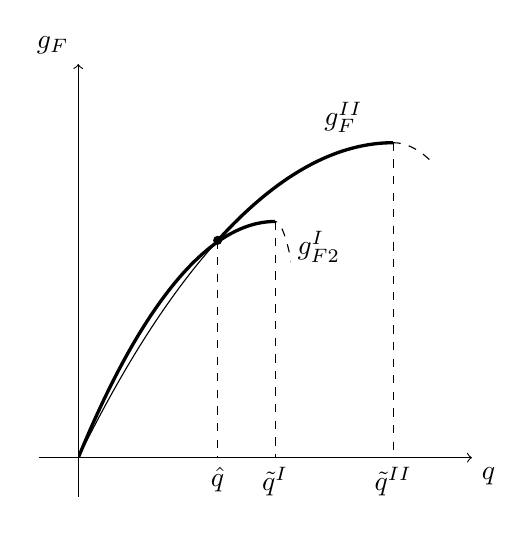
\begin{tikzpicture}
\draw[->] (-0.5, 0) -- (5, 0) node[below right] {$q$};
\draw[->] (0, -0.5) -- (0, 5) node[above left]  {$g_F$};
\begin{scope}
	\clip (0, 0) rectangle (1.95, 2.98);
	\draw(0, 0) parabola bend (4, 4) (6, 0);
\end{scope}
\begin{scope}
	\clip (1.77, 2.7) rectangle (4, 5);
	\draw[style=very thick] (0, 0) parabola bend (4, 4) (6, 0);
\end{scope}
\draw (3, 4) node [above right] {$g^{II}_{F}$};
\begin{scope}
	\clip (4, 0) rectangle (4.5, 5);
	\draw[style=dashed] (0, 0) parabola bend (4, 4) (6, 0);
\end{scope}
\begin{scope}
	\clip (0, 0) rectangle (2.5, 4);
	\draw[style=very thick] (0, 0) parabola bend (2.5, 3) (3, 0);
\end{scope}
\begin{scope}
	\clip (2.5, 0) rectangle (2.7, 3);
	\draw[style=dashed] (0, 0) parabola bend (2.5, 3) (3, 0);
\end{scope}
\filldraw (1.77, 2.76) circle (0.05);
\draw (3.45, 3) node [below left] {$g^{I}_{F2}$};
\draw[style=dashed] (1.77, 2.76) -- (1.77, 0) node[below] {$\hat{q}$};
\draw[style=dashed] (2.5, 3) -- (2.5, 0) node[below] {$\tilde{q}^{I}$};
\draw[style=dashed] (4, 4) -- (4, 0) node[below] {$\tilde{q}^{II}$};
\end{tikzpicture}
\end{document}
